% ============================================================
%  Advanced Embedded Systems Lab — Final Documentation
%  Team A3 | Summer Term 2025
% ============================================================
\documentclass[11pt,a4paper]{article}

\usepackage[T1]{fontenc}
\usepackage[utf8]{inputenc}
\usepackage{lmodern}
\usepackage[english]{babel}
\usepackage{geometry}
\geometry{a4paper, top=2.5cm, bottom=2.5cm, left=2.5cm, right=2.5cm}
\usepackage{graphicx}
\usepackage{xcolor}
\usepackage{booktabs}
\usepackage{array}
\usepackage{tabularx}
\usepackage{float}
\usepackage{hyperref}
\usepackage{fancyhdr}
\usepackage{titlesec}
\usepackage{enumitem}
\usepackage{amsmath}
\usepackage{caption}
\usepackage{setspace}
\usepackage{parskip}
\usepackage{microtype}
\usepackage{tcolorbox}
\usepackage{tikz}
\usetikzlibrary{shapes.geometric, arrows.meta, positioning, automata}

\definecolor{primaryblue}{RGB}{0,70,140}
\definecolor{accentgray}{RGB}{90,90,90}
\definecolor{lightgray}{RGB}{245,245,245}
\definecolor{passgreen}{RGB}{0,140,60}
\definecolor{blockgray}{RGB}{220,228,240}

\hypersetup{colorlinks=true, linkcolor=primaryblue, urlcolor=primaryblue}

\pagestyle{fancy}
\fancyhf{}
\fancyhead[L]{\small Hardware Engineering Lab}
\fancyhead[R]{\small Summer term 2026}
\fancyfoot[C]{\thepage}
\renewcommand{\headrulewidth}{0.4pt}

\titleformat{\section}
  {\normalfont\Large\bfseries\color{primaryblue}}{\thesection}{1em}{}[{\titlerule[0.4pt]}]
\titleformat{\subsection}
  {\normalfont\normalsize\bfseries\color{accentgray}}{\thesubsection}{1em}{}

\newcolumntype{C}[1]{>{\centering\arraybackslash}p{#1}}
\newcolumntype{L}[1]{>{\raggedright\arraybackslash}p{#1}}

\newtcolorbox{notebox}{colback=lightgray, colframe=primaryblue,
  fonttitle=\bfseries, left=4pt, right=4pt, top=3pt, bottom=3pt}

% ── TikZ styles for FSM diagram ──────────────────────────────
\tikzset{
  state/.style={
    draw, circle, minimum size=1.3cm,
    fill=blockgray, font=\small\bfseries,
    line width=0.8pt
  },
  arrow/.style={-{Stealth[length=6pt]}, line width=0.7pt},
  label/.style={font=\footnotesize, fill=white, inner sep=1pt}
}

% ── TikZ styles for block diagram ───────────────────────────
\tikzset{
  block/.style={
    draw, rectangle, rounded corners=3pt,
    minimum width=2.6cm, minimum height=0.75cm,
    fill=blockgray, font=\small, align=center,
    line width=0.7pt
  },
  smallblock/.style={
    draw, rectangle, rounded corners=2pt,
    minimum width=2cm, minimum height=0.6cm,
    fill=white, font=\footnotesize, align=center,
    line width=0.6pt
  },
  wire/.style={-{Stealth[length=5pt]}, line width=0.6pt}
}

% ============================================================
\begin{document}
\setlength{\parskip}{5pt}

% ── Title block ─────────────────────────────────────────────
\begin{center}
  {\LARGE\bfseries Technical Report Hardware Engineering}\\[0.35cm]
  {\large\bfseries Team A3}\\[0.15cm]
  {\large\today}
\end{center}

\vspace{0.3cm}
\tableofcontents


% ============================================================
\section*{Team Members}
\addcontentsline{toc}{section}{Team Members}
% ============================================================

\begin{center}
\begin{tabular}{lll}
  \toprule
  \textbf{Name} & \textbf{Role} & \textbf{Sections authored} \\
  \midrule
  Rionela Kovaci    & VHDL Design, Schematic      & Introduction, Concept description, Technologies \\
  Christian Percival & PCB Layout \& Routing       & Implementation (PCB), Results \\
  Mohamed Abdo      & ALU / FSM, DRC \& Compliance & Implementation (VHDL/FSM), Sources \\
  \bottomrule
\end{tabular}
\end{center}

% ============================================================
\section{Introduction}
% ============================================================

This report documents the complete hardware design project realised by Team~A3
during the Hardware Engineering Lab, Summer Term 2026. The project is
composed of two tightly coupled parts:

\begin{enumerate}[leftmargin=2em, noitemsep]
  \item \textbf{VHDL soft-core CPU on Nexys A7 (Vivado)} — an 8-bit
        register-based CPU with a multi-operation ALU, implemented in VHDL and
        synthesised for an Artix-7 FPGA using Xilinx Vivado. The system
        supports addition, subtraction, multiplication, and division, with
        results displayed in signed decimal on a seven-segment display.

  \item \textbf{Custom PCB design (Altium)} — a four-layer printed
        circuit board built around a Lattice iCE40UP5K-SG48I FPGA, designed to
        take the prototyped logic from the development board to a real,
        manufacturable hardware platform.
\end{enumerate}

Together, the two parts demonstrate the full embedded-hardware development
cycle: \emph{design and verify in simulation $\rightarrow$ prototype on FPGA
dev-board $\rightarrow$ tape-out to custom PCB}.

% ============================================================
\section{Concept Description}
% ============================================================

\subsection{System overview}

The VHDL project implements a simple but complete \textbf{8-bit CPU} on a
Nexys A7 development board. The user interacts entirely through the board's
switches, push-buttons, and seven-segment display — no PC connection is needed
during operation.

\begin{figure}[H]
\centering
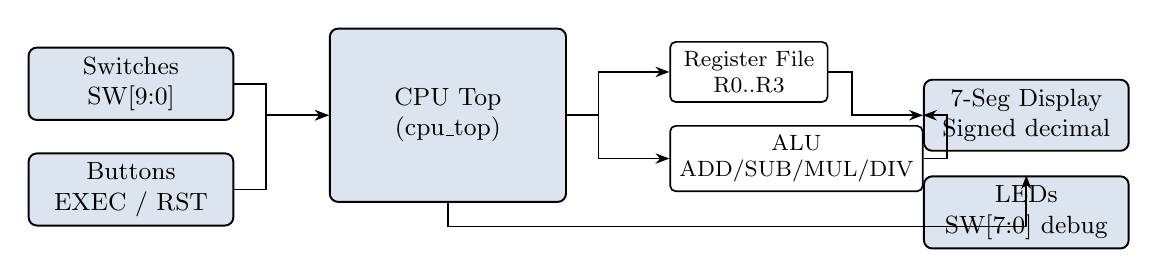
\begin{tikzpicture}[node distance=0.5cm and 0.8cm]
  % Input column
  \node[block] (sw)  {Switches\\SW[9:0]};
  \node[block, below=0.4cm of sw]  (btn) {Buttons\\EXEC / RST};

  % CPU core
  \node[block, right=1.2cm of sw, yshift=-0.4cm,
        minimum height=2.2cm, minimum width=3cm] (cpu) {CPU Top\\(cpu\_top)};

  % Internals
  \node[smallblock, right=1.3cm of cpu, yshift=0.55cm]  (rf)  {Register File\\R0..R3};
  \node[smallblock, right=1.3cm of cpu, yshift=-0.55cm] (alu) {ALU\\ADD/SUB/MUL/DIV};

  % Output column
  \node[block, right=1.2cm of rf,  yshift=-0.55cm] (seg) {7-Seg Display\\Signed decimal};
  \node[block, below=0.3cm of seg] (led) {LEDs\\SW[7:0] debug};

  % Wires
  \draw[wire] (sw.east)  -- ++(0.4,0) |- (cpu.west);
  \draw[wire] (btn.east) -- ++(0.4,0) |- (cpu.west);
  \draw[wire] (cpu.east) -- ++(0.4,0) |- (rf.west);
  \draw[wire] (cpu.east) -- ++(0.4,0) |- (alu.west);
  \draw[wire] (rf.east)  -- ++(0.3,0) |- (seg.west);
  \draw[wire] (alu.east) -- ++(0.3,0) |- (seg.west);
  \draw[wire] (cpu.south) -- ++(0,-0.3) -| (led.north);
\end{tikzpicture}
\caption{Top-level block diagram of the VHDL CPU system}
\label{fig:block}
\end{figure}

\subsection{Main application}

The prototype is an \textbf{interactive 8-bit calculator} with a four-register
file. The user loads signed 8-bit values into registers R0–R3 and executes
arithmetic operations (ADD, SUB, MUL, DIV) between any two registers, storing
the result in a destination register. Results are displayed in signed decimal
(range $-128$ to $+127$) on the seven-segment display. Division results are
shown as \emph{quotient.remainder} using the decimal point.

\subsection{Components and interfaces}

\begin{center}
\begin{tabularx}{\linewidth}{L{3.5cm}L{9cm}}
  \toprule
  \textbf{Component} & \textbf{Description} \\
  \midrule
  Nexys A7 board      & Artix-7 FPGA development board; hosts the entire VHDL design \\
  SW[9:0]             & 10 slide-switches: mode, sign, magnitude, register select, operation \\
  btn\_exec           & Edge-triggered execute button (load or run ALU) \\
  btn\_rst            & Asynchronous reset; clears all registers and CPU state \\
  7-segment display   & 8-digit multiplexed display; shows signed result and remainder \\
  LEDs [7:0]          & Mirror SW[7:0] for live switch-state debugging \\
  Lattice iCE40UP5K   & FPGA on the custom PCB (Part 2 of the project) \\
  \bottomrule
\end{tabularx}
\end{center}

% ============================================================
\section{Project / Team Management}
% ============================================================

\subsection{Development workflow}

The team followed a two-phase hardware development flow:

\begin{enumerate}[leftmargin=2em]
  \item \textbf{VHDL phase} — architecture definition, RTL coding in VHDL,
        functional simulation in Vivado, synthesis and implementation for
        Artix-7, on-board testing with Nexys A7.
  \item \textbf{PCB phase} — schematic capture in Altium Designer, four-layer
        layout, DRC verification, and Gerber export to JLCPCB production
        standards.
\end{enumerate}

\subsection{Task distribution}

\begin{center}
\begin{tabularx}{\linewidth}{L{3.2cm}L{3cm}L{7.5cm}}
  \toprule
  \textbf{Task} & \textbf{Owner} & \textbf{Details} \\
  \midrule
  CPU architecture    & Rionela Kovaci    & Top-level entity, register file, mode/switch decode \\
  ALU design          & Mohamed Abdo      & ADD, SUB, MUL, DIV; FSM control; carry/overflow/div-zero flags \\
  Display subsystem   & Rionela Kovaci    & BCD conversion, 7-seg decoder, multiplexed refresh, signed/div display \\
  Vivado flow         & Mohamed Abdo      & Synthesis, implementation, constraints, bitstream \\
  PCB schematic       & Rionela Kovaci    & FPGA, power supply, SPI Flash, UI peripherals \\
  PCB layout \& route & Christian Percival & 4-layer stack-up, autoroute, serpentine tuning \\
  DRC \& compliance   & Christian Percival & Via rules, JLCPCB verification, Gerber export \\
  Documentation       & All members       & Per-section authorship (see Team Members table) \\
  \bottomrule
\end{tabularx}
\end{center}

% ============================================================
\section{Technologies}
% ============================================================

\subsection{VHDL and Vivado}

The CPU is described entirely in \textbf{VHDL} (VHSIC Hardware Description
Language) at the register-transfer level (RTL). Xilinx \textbf{Vivado
2024.x} was used for synthesis, implementation, and bitstream generation
targeting the \textbf{Artix-7 XC7A100T} on the Nexys A7 board. Functional
verification was performed with Vivado's built-in simulator before programming
the board.

\subsection{Hardware description: cpu\_top architecture}

The top-level entity \texttt{cpu\_top} instantiates three sub-components and
contains the complete datapath and control logic:

\begin{itemize}[leftmargin=2em, noitemsep]
  \item \textbf{\texttt{alu}} — arithmetic logic unit with a clocked FSM
        (described in Section~\ref{sec:impl}).
  \item \textbf{\texttt{binary\_to\_bcd}} — double-dabble converter producing
        hundreds, tens, and ones BCD digits from an 8-bit binary value.
  \item \textbf{\texttt{seven\_segment\_decoder}} — combinational 4-to-7
        segment decoder; instantiated four times (ones, tens, hundreds,
        remainder-ones).
\end{itemize}

\subsection{Switch interface encoding}

\begin{center}
\begin{tabularx}{\linewidth}{C{2cm}C{2cm}L{8.5cm}}
  \toprule
  \textbf{Mode} & \textbf{Switch} & \textbf{Function} \\
  \midrule
  Both   & SW[8]     & 0 = Load mode, 1 = Execute mode \\
  Load   & SW[7]     & Sign: 0 = positive, 1 = negative (two's complement applied) \\
  Load   & SW[3:0]   & 4-bit magnitude (0–15) \\
  Load   & SW[5:4]   & Destination register R0–R3 \\
  Execute & SW[7:6]  & Operation: 00=ADD, 01=SUB, 10=MUL, 11=DIV \\
  Execute & SW[1:0]  & Source register A (R0–R3) \\
  Execute & SW[3:2]  & Source register B (R0–R3) \\
  Execute & SW[5:4]  & Destination register R0–R3 \\
  \bottomrule
\end{tabularx}
\end{center}

\subsection{PCB tools and FPGA}

The custom PCB was designed in \textbf{Altium Designer} around the
\textbf{Lattice iCE40UP5K-SG48I} FPGA. Power is supplied through two
\textbf{AMS1117} LDO regulators (3.3\,V and 1.2\,V), with configuration
stored in a \textbf{Winbond W25Q16} SPI NOR Flash. The board was verified
against \textbf{JLCPCB} manufacturing constraints and exported as Gerber files.

% ============================================================
\section{Implementation}
\label{sec:impl}
% ============================================================

\subsection{CPU finite-state machine (FSM)}

The CPU control logic operates as a two-state Mealy FSM clocked on the
rising edge of \texttt{clk}, with asynchronous reset on \texttt{btn\_rst}.

\begin{figure}[H]
\centering
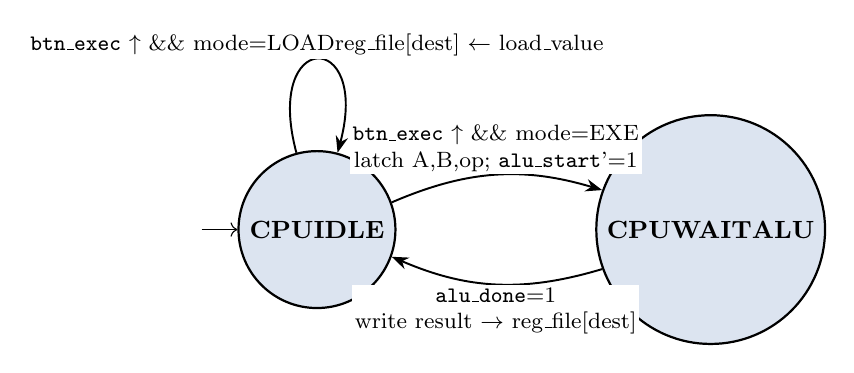
\begin{tikzpicture}[node distance=5cm, on grid]
  \node[state, initial, initial text={}] (idle) {CPU\\IDLE};
  \node[state, right=of idle]           (wait) {CPU\\WAIT\\ALU};

  % IDLE -> WAIT
  \draw[arrow] (idle) to[bend left=20]
    node[label, above, align=center]
      {\texttt{btn\_exec} $\uparrow$ \&\& mode=EXE\\
       latch A,B,op; \texttt{alu\_start}'=1}
    (wait);

  % WAIT -> IDLE
  \draw[arrow] (wait) to[bend left=20]
    node[label, below, align=center]
      {\texttt{alu\_done}=1\\
       write result $\rightarrow$ reg\_file[dest]}
    (idle);

  % Self-loop IDLE (load)
  \draw[arrow] (idle) to[loop above]
    node[label, above]{\texttt{btn\_exec} $\uparrow$ \&\& mode=LOAD\\
                        reg\_file[dest] $\leftarrow$ load\_value}
    (idle);
\end{tikzpicture}
\caption{CPU top-level FSM — two states, edge-triggered execute button}
\label{fig:fsm}
\end{figure}

\textbf{State descriptions:}

\textbf{CPU\_IDLE} — the CPU waits for a rising edge on \texttt{btn\_exec}
(detected by comparing \texttt{btn\_exec} with the registered
\texttt{btn\_prev}). In \emph{Load mode} (SW[8]=0), the switch-encoded signed
value is written directly into the selected register; the ALU is not involved.
In \emph{Execute mode} (SW[8]=1), operands A and B are latched into
\texttt{alu\_a\_reg} and \texttt{alu\_b\_reg}, the operation code into
\texttt{alu\_op\_reg}, and \texttt{alu\_start} is pulsed for one clock cycle
before transitioning to CPU\_WAIT\_ALU.

\textbf{CPU\_WAIT\_ALU} — the CPU holds until \texttt{alu\_done} is asserted
by the ALU. On that cycle, the ALU result is written to the destination
register, and the flags (overflow, div\_zero, remainder) are captured into
registered signals for display. The FSM returns to CPU\_IDLE.

\subsection{ALU operations and flags}

The ALU implements four operations selected by \texttt{op[1:0]}:

\begin{center}
\begin{tabular}{cll}
  \toprule
  \textbf{op} & \textbf{Operation} & \textbf{Notes} \\
  \midrule
  00 & ADD & 8-bit signed; carry and overflow flags set \\
  01 & SUB & Implemented as ADD with two's complement of B \\
  10 & MUL & 8-bit $\times$ 8-bit; lower 8 bits stored as result \\
  11 & DIV & Quotient in result, remainder in \texttt{alu\_remainder}; div\_zero flag on B=0 \\
  \bottomrule
\end{tabular}
\end{center}

Two utility functions defined in \texttt{cpu\_top} support arithmetic:
\texttt{add8\_ci} performs a ripple-carry 8-bit addition with carry-in, and
\texttt{twos\_comp8} computes the two's complement by inverting all bits and
adding 1 via \texttt{add8\_ci}.

\subsection{Display subsystem}

The seven-segment display is driven by a \textbf{time-multiplexed refresh
process} cycling through four digit positions at 50\,kHz (refresh counter
rolls at 49\,999 clock cycles). Three display modes are handled:

\begin{itemize}[leftmargin=2em, noitemsep]
  \item \textbf{Normal signed} — digits show the selected register value in
        decimal with a leading minus sign placed in the correct position
        (e.g.\ $-128$ fills all four digits; $-5$ shows just \texttt{-5}).
  \item \textbf{Division} (\texttt{stored\_op=11}) — quotient is shown with
        a decimal point separating it from the remainder digit (e.g.\
        \texttt{12.3} means quotient 12, remainder 3).
  \item \textbf{Error (OF)} — when overflow or divide-by-zero is detected,
        the display shows \texttt{OF} using custom segment constants
        \texttt{SEG\_O} and \texttt{SEG\_F}.
\end{itemize}

\subsection{PCB implementation — 4-layer stack-up}

\begin{table}[H]
  \centering
  \caption{PCB Layer Stack-Up}
  \begin{tabularx}{\linewidth}{C{1cm}L{3cm}C{2.2cm}L{7cm}}
    \toprule
    \textbf{Layer} & \textbf{Function} & \textbf{Thickness} & \textbf{Purpose} \\
    \midrule
    L1 & Top — Signals + Components & 1.4\,mil   & FPGA, regulators, SPI Flash, UI \\
    L2 & GND Plane                  & 1.378\,mil & Solid copper pour — EMI shield, return path \\
    L3 & VCC\_3.3\,V Plane          & 1.378\,mil & Power distribution, minimal routing \\
    L4 & Bottom — Signals + Caps    & 1.4\,mil   & Return signals, decoupling caps C1–C11 \\
    \bottomrule
  \end{tabularx}
\end{table}

\subsection{Decoupling capacitor strategy}

\begin{table}[H]
  \centering
  \caption{Decoupling Capacitor Assignment}
  \begin{tabularx}{\linewidth}{C{2.5cm}C{2cm}L{8cm}}
    \toprule
    \textbf{Reference} & \textbf{Value} & \textbf{Function} \\
    \midrule
    C1 – C8      & 100\,nF     & FPGA VCC\_3.3\,V \& VCC\_1.2\,V decoupling \\
    C9 – C11     & 100\,nF     & USB\_5\,V input line filtering \\
    CB\_1, CB\_2 & 4.7\,$\mu$F & Bulk capacitors on 3.3\,V and 1.2\,V rails \\
    C\_F         & 100\,nF     & SPI Flash VCC bypass \\
    \bottomrule
  \end{tabularx}
\end{table}

All capacitors are placed \textbf{within 2\,mm of their associated FPGA power
pin} on the bottom layer, minimising parasitic inductance.

\subsection{Trace widths and via rules}

\begin{table}[H]
  \centering
  \caption{Trace Width and Via Design Rules vs.\ JLCPCB Minimums}
  \begin{tabularx}{\linewidth}{L{2.5cm}C{2cm}C{2.5cm}C{2.5cm}C{1cm}}
    \toprule
    \textbf{Net / Via} & \textbf{JLCPCB Min} & \textbf{Industry Std} & \textbf{Our Design} & \textbf{Pass} \\
    \midrule
    \multicolumn{5}{l}{\textit{Trace widths}} \\
    GND          & 5\,mil & 15–25\,mil & 20\,mil & \textcolor{passgreen}{\checkmark} \\
    USB 5\,V     & 5\,mil & 20–30\,mil & 24\,mil & \textcolor{passgreen}{\checkmark} \\
    VCC 3.3\,V   & 5\,mil & 12–20\,mil & 16\,mil & \textcolor{passgreen}{\checkmark} \\
    VCC 1.2\,V   & 5\,mil & 10–15\,mil & 12\,mil & \textcolor{passgreen}{\checkmark} \\
    Signals      & 5\,mil & 6–10\,mil  & 8\,mil  & \textcolor{passgreen}{\checkmark} \\
    \midrule
    \multicolumn{5}{l}{\textit{Via dimensions (hole / pad)}} \\
    Signal vias  & 0.3 / 0.5\,mm & 0.3 / 0.6\,mm & 12 / 24\,mil & \textcolor{passgreen}{\checkmark} \\
    VCC 3.3\,V   & 0.3 / 0.5\,mm & 0.4 / 0.8\,mm & 16 / 28\,mil & \textcolor{passgreen}{\checkmark} \\
    Power GND    & 0.3 / 0.5\,mm & 0.45 / 0.9\,mm& 18 / 32\,mil & \textcolor{passgreen}{\checkmark} \\
    USB 5\,V     & 0.3 / 0.5\,mm & 0.45 / 0.9\,mm& 18 / 32\,mil & \textcolor{passgreen}{\checkmark} \\
    Annular ring & 0.1\,mm       & 0.15\,mm       & 6\,mil       & \textcolor{passgreen}{\checkmark} \\
    \bottomrule
  \end{tabularx}
\end{table}

\subsection{Routing and serpentine length tuning}

The board was routed with the Situs autorouter (shortest-path, 6\,mil
clearance). Critical nets — \texttt{CLK\_12M} and all three SPI Flash lines
(\texttt{FLASH\_SCK}, \texttt{FLASH\_SI}, \texttt{FLASH\_SO}) — were then
\textbf{length-matched} using Altium's Interactive Length Tuning
(\texttt{Shift+A}) to eliminate propagation skew across the parallel bus.
Settings: amplitude 0.3–0.5\,mm, gap 0.15\,mm, rounded corners. The result
was \textbf{0 DRC violations} after tuning.

\begin{figure}[H]
  \centering
  \includegraphics[width=\linewidth]{Layout.png}
  \caption{PCB layout}
  \label{fig:serpentine}
\end{figure}

% ============================================================
\section{Results}
% ============================================================

\subsection{VHDL simulation and on-board testing}

The complete CPU was simulated in Vivado before synthesis. All four ALU
operations were verified with both positive and negative operands. Edge cases
tested include:
\begin{itemize}[leftmargin=2em, noitemsep]
  \item Signed overflow: e.g.\ $127 + 1$ triggers the \texttt{overflow} flag
        and displays \texttt{OF}.
  \item Division by zero: B=0 triggers \texttt{div\_zero}, display shows
        \texttt{OF}.
  \item Division display: e.g.\ $25 \div 4$ shows \texttt{6.1} (quotient 6,
        remainder 1) with the decimal point active.
  \item Negative display: e.g.\ $-128$ correctly drives all four digit
        positions including the leading minus.
\end{itemize}

After synthesis and programming, all cases were confirmed on the Nexys A7
board.

\subsection{PCB manufacturing compliance}

\begin{table}[H]
  \centering
  \caption{JLCPCB Manufacturing Compliance}
  \begin{tabularx}{\linewidth}{Xccc}
    \toprule
    \textbf{Parameter} & \textbf{JLCPCB Min} & \textbf{Industry Std} & \textbf{Our Design} \\
    \midrule
    Min trace width      & 5\,mil (0.127\,mm)  & 6–8\,mil    & 8\,mil \\
    Min clearance        & 5\,mil (0.127\,mm)  & 6\,mil      & 6\,mil \\
    Via hole (signal)    & 0.3\,mm (11.8\,mil) & 0.3\,mm     & 12\,mil (0.305\,mm) \\
    Via pad (signal)     & 0.5\,mm (19.7\,mil) & 0.6\,mm     & 24\,mil (0.61\,mm) \\
    Annular ring         & 0.1\,mm (3.94\,mil) & 0.15\,mm    & 6\,mil (0.15\,mm) \\
    Power trace (3.3\,V) & 5\,mil min          & 12–20\,mil  & 16\,mil \\
    Power trace (GND)    & 5\,mil min          & 15–25\,mil  & 20\,mil \\
    Hole-to-hole spacing & 0.5\,mm edge        & 0.5\,mm     & Verified via DRC \\
    Layer count          & Standard 4-layer    & 4-layer     & 4 layers \\
    \bottomrule
  \end{tabularx}
  \label{tab:compliance}
\end{table}

\subsection{DRC result — 0 violations}

\begin{center}
  \begin{tcolorbox}[colback=passgreen!10, colframe=passgreen,
      width=0.55\linewidth, halign=center, fontupper=\large\bfseries]
    DRC Result: \textcolor{passgreen}{0 Violations}
  \end{tcolorbox}
\end{center}

\vspace{0.2cm}
All five DRC categories confirmed clear:
\begin{itemize}[leftmargin=2em, noitemsep]
  \item[\textcolor{passgreen}{\checkmark}] Clearance: 0 violations
  \item[\textcolor{passgreen}{\checkmark}] Short-circuit: 0 violations
  \item[\textcolor{passgreen}{\checkmark}] Un-routed nets: 0 violations
  \item[\textcolor{passgreen}{\checkmark}] Net antennae: 0 violations
  \item[\textcolor{passgreen}{\checkmark}] Hole-to-hole: 0 violations
\end{itemize}

The Gerber files are ready for production submission to JLCPCB.

% ============================================================
\section*{Sources / References}
\addcontentsline{toc}{section}{Sources / References}
% ============================================================

\begin{enumerate}[leftmargin=2em, label={[\arabic*]}]
  \item Xilinx/AMD, \textit{Vivado Design Suite User Guid,, Synthesis},
        UG901, \url{https://docs.amd.com}.
  \item \small{Digilent, \textit{Nexys A7 Reference Manual},
        \url{https://digilent.com/reference/programmable-logic/nexys-a7}.}
  \item JLCPCB, \textit{PCB Manufacturing Capabilities},
        \url{https://jlcpcb.com/capabilities/pcb-capabilities}.
  \item \small{Lattice Semiconductor, \textit{iCE40 UltraPlus Family Data Sheet},
        \url{https://www.latticesemi.com}.}
  \item Winbond Electronics, \textit{W25Q16JV Serial NOR Flash Data Sheet},
        2018.
  \item AMS, \textit{AMS1117 LDO Voltage Regulator Data Sheet}, 2020.
  \item Altium, \textit{Interactive Length Tuning — Altium Designer Docs},
        \url{https://www.altium.com/documentation/altium-designer}.
  \item Team A3, \textit{Project}, GitHub:
        \url{https://github.com/MoAbdoHSHL/Hardware-Engineering-Gr_A3/tree/main}.
\end{enumerate}

\end{document}
